\chapter{Introduction to Using Tensorflow}
\section{Template for Experiments}
The template followed for all experiments in chapters three, four and five is outlined in Figure \ref{fig:expTemplate}.

\begin{table}[]
\centering
\caption{Experiment Template}
\label{fig:expTemplate}
\begin{tabular}{ll}
Experiment Section   & Rationale                \\
Overview             & An explanation of the purpose of the experiment along with how it is carried out. \\
Network Architecture & An explanation of the network architecture used in the experiment. If the architecture has been explained in another experiment, the architecture will only be referenced by name.                       \\
Dataset              & The dataset used for the experiment, with its source and an overview of its details. A brief mention will be made in following experiments.                       \\
API's                & Reference to the technologies used as outlined in Chapter 2.                      \\
Script               & Snippets of the script used for the experiment.                       \\
Results              & The results acquired from the experiment, usually in the form of a percentage accuracy.                       \\
Empirical Analysis   & States any information gained from the experiment and speculation for the reasoning of the results.                      
\end{tabular}
\end{table}

\section{Udemy Tutorial}
\label{udemy1}
\subsection*{Overview}
There are many on line resources that are geared towards helping deep learning novices.
One of these resources is a course on Udemy titled 'Complete Guide to Tensorflow for Deep Learning with Python' \textcite{udemy}.
This course has a section on Convolutional Neural Networks which has been followed and completed.

\subsection*{Network Architecture}
The architecture for this network is very simple as it is an introductory CNN.
It consists of two convolutional layers, two max pooling layers and a fully connected layer.

\subsection*{Dataset}
This CNN is trained on the MNIST dataset.
This dataset consists of 70000 handwritten digits \textcite{mnist}.

\subsection*{API's}
This experiment was carried out in a jupyter notebook using tensorflow.

\subsection*{Script}
\begin{lstlisting}

#Helper Functions

#INIT WEIGHTS
def init_weights(shape):
    init_random_dist = tf.truncated_normal(shape, stddev = 0.1)
    return tf.Variable(init_random_dist)

#INIT BIAS
def init_bias(shape):
    init_bias_vals = tf.constant(0.1, shape = shape)
    return tf.Variable(init_bias_vals)

#CONV2D
def conv2d(x, W):
    #x -> [batch, H, W, Channels]
    #W -> [filterH, filterW, ChannelsIn, ChannelsOut]
    return tf.nn.conv2d(x, W, strides = [1,1,1,1], padding = 'SAME')

#POOLING
def max_pool_2by2(x):
    #x -> [batch, H, W, Channels]
    return tf.nn.max_pool(x, ksize = [1,2,2,1], strides = [1,2,2,1], padding = 'SAME')

    #NORMAL (FULLY CONNECTED)
def normal_full_layer(input_layer, size):
    input_size = int(input_layer.get_shape()[1])
    W = init_weights([input_size, size])
    b = init_bias([size])
return tf.matmul(input_layer, W) + b
\end{lstlisting}

\begin{lstlisting}
#32 features for every 5 x 5 patch with 1(grayscale)
convo_1 = convolutional_layer(x_image, shape = [5,5,1,32])
convo_1_pooling = max_pool_2by2(convo_1)

convo_2 = convolutional_layer(convo_1_pooling, shape = [5,5,32,64])
convo_2_pooling = max_pool_2by2(convo_2)

convo_2_flat = tf.reshape(convo_2_pooling, [-1,7*7*64])
full_layer_one = tf.nn.relu(normal_full_layer(convo_2_flat, 1024))
\end{lstlisting}

\begin{lstlisting}
with tf.Session() as sess:
    sess.run(init)
    
    for i in range(steps):
        batch_x, batch_y = mnist.train.next_batch(32)
        batch_test = mnist.test.next_batch(32)
        sess.run(train, feed_dict = {x:batch_x, y_true:batch_y, hold_prob:0.5})
        if i%500 == 0:
            print("ON STEP: {}".format(i))
            print("ACCURACY: ")
            match = tf.equal(tf.argmax(y_pred, 1), tf.argmax(y_true, 1))
            acc = tf.reduce_mean(tf.cast(match, tf.float32))
            print(sess.run(acc, feed_dict = {x:batch_test, y_true:mnist.test.labels, hold_prob:1.0}))
            print('\n')
            
    sess.run(acc, feed_dict = {x:mnist.test.images} )

#Final Accuracy 0.973
\end{lstlisting}

\subsection*{Results}
The Final Accuracy for this experiment was of 97.3\%.


\section{Udemy Tutorial 2}
\label{udemy2}
\subsection*{Objective}
Similar to the previous experiment \ref{udemy2}, this experiment is a Udemy course exercise \parencite{udemy}. In contrast, this does not use a dataset built into TensorFlow so therefore, there is extra configuration to be done on the dataset.

\subsection*{Network Architecture}
Same architecture as in \ref{udemy1}.

\subsection*{Dataset}
The CIFAR-10 dataset is used here. 
This has 60000 images split into 10 classes and a test set of 1000 images \parencite{cifar}.

\subsection*{Script}
\begin{lstlisting}[style=Python]
def unpickle(file):
    import pickle
    with open(file, 'rb') as fo:
        cifar_dict = pickle.load(fo, encoding='bytes')
    return cifar_dict

dirs = ['batches.meta','data_batch_1','data_batch_2','data_batch_3','data_batch_4','data_batch_5','test_batch']

all_data = [0,1,2,3,4,5,6]

for i,direc in zip(all_data,dirs):
    all_data[i] = unpickle(CIFAR_DIR+direc)

batch_meta = all_data[0]
data_batch1 = all_data[1]
data_batch2 = all_data[2]
data_batch3 = all_data[3]
data_batch4 = all_data[4]
data_batch5 = all_data[5]
test_batch = all_data[6]
\end{lstlisting}

\begin{lstlisting}[style=Python]
def set_up_images(self):
        
        print("Setting Up Training Images and Labels")
        
        # Vertically stacks the training images
        self.training_images = np.vstack([d[b"data"] for d in self.all_train_batches])
        train_len = len(self.training_images)
        
        # Reshapes and normalizes training images
        self.training_images = self.training_images.reshape(train_len,3,32,32).transpose(0,2,3,1)/255
        # One hot Encodes the training labels (e.g. [0,0,0,1,0,0,0,0,0,0])
        self.training_labels = one_hot_encode(np.hstack([d[b"labels"] for d in self.all_train_batches]), 10)
        
        print("Setting Up Test Images and Labels")
        
        # Vertically stacks the test images
        self.test_images = np.vstack([d[b"data"] for d in self.test_batch])
        test_len = len(self.test_images)
        
        # Reshapes and normalizes test images
        self.test_images = self.test_images.reshape(test_len,3,32,32).transpose(0,2,3,1)/255
        # One hot Encodes the test labels (e.g. [0,0,0,1,0,0,0,0,0,0])
        self.test_labels = one_hot_encode(np.hstack([d[b"labels"] for d in self.test_batch]), 10)

        
    def next_batch(self, batch_size):
        # Note that the 100 dimension in the reshape call is set by an assumed batch size of 100
        x = self.training_images[self.i:self.i+batch_size].reshape(100,32,32,3)
        y = self.training_labels[self.i:self.i+batch_size]
        self.i = (self.i + batch_size) % len(self.training_images)
return x, y
\end{lstlisting}

\begin{lstlisting}[style=Python]
cross_entropy = tf.reduce_mean(tf.nn.softmax_cross_entropy_with_logits(labels = y_true, logits = y_pred))
optimizer = tf.train.AdamOptimizer(learning_rate = 0.001)
train = optimizer.minimize(cross_entropy)
init = tf.global_variables_initializer()
with tf.Session() as sess:
    sess.run(tf.global_variables_initializer())

    for i in range(10000):
        batch = ch.next_batch(100)
        sess.run(train, feed_dict={x: batch[0], y_true: batch[1], hold_prob: 0.5})
        
        # PRINT OUT A MESSAGE EVERY 100 STEPS
        if i%1000 == 0:
            
            # Test the Train Model
            matches = tf.equal(tf.argmax(y_pred,1),tf.argmax(y_true,1))

            acc = tf.reduce_mean(tf.cast(matches,tf.float32))
            testSet = ch.next_test_batch(100)
            print('Accuracy: ')
            print(sess.run(acc,feed_dict={x:testSet[0] ,y_true:testSet[1],hold_prob:1.0}))
print('\n')
\end{lstlisting}

\subsection*{Results}
A Final Accuracy of 71\% was reached.

\subsection*{Analysis}


\section{Using the Food 101 dataset}
\label{food101}
\subsection*{Objective}
For the next experiment, it was decided to use the Food-101 dataset.
An on line tutorial was used to create a dataset in TensorFlow using image directories on disk \parencite{file_dir_code}.
Tutorials used previously were also utilized for this experiment \parencite{udemy} and \parencite{cifar}.

\subsection*{Network Architecture}
A similar network architecture to the previous two experiments (\ref{udemy1} and \ref{udemy2}) was used here.

\subsection*{Dataset}
The Food-101 dataset was used for this experiment \parencite{food101}.

\subsection*{Script}
\begin{lstlisting}[style=Python]
# Reading the dataset
# 2 modes: 'file' or 'folder'
def read_images(dataset_path, mode, batch_size):
    imagepaths, labels = list(), list()
    if mode == 'file':
        # Read dataset file
        data = open(dataset_path, 'r').read().splitlines()
        for d in data:
            imagepaths.append(d.split(' ')[0])
            labels.append(int(d.split(' ')[1]))
    elif mode == 'folder':
        # An ID will be affected to each sub-folders by alphabetical order
        label = 0
        # List the directory
        try:  # Python 2
            classes = sorted(os.walk(dataset_path).next()[1])
        except Exception:  # Python 3
            classes = sorted(os.walk(dataset_path).__next__()[1])
        # List each sub-directory (the classes)
        for c in classes:
            c_dir = os.path.join(dataset_path, c)
            try:  # Python 2
                walk = os.walk(c_dir).next()
            except Exception:  # Python 3
                walk = os.walk(c_dir).__next__()
            # Add each image to the training set
            for sample in walk[2]:
                # Only keeps jpeg images
                if sample.endswith('.jpg') or sample.endswith('.jpeg'):
                    imagepaths.append(os.path.join(c_dir, sample))
                    labels.append(label)
            label += 1
    else:
raise Exception("Unknown mode.")
\end{lstlisting}

\begin{lstlisting}[style=Python]
# Convert to Tensor
    imagepaths = tf.convert_to_tensor(imagepaths, dtype=tf.string)
    labels = tf.convert_to_tensor(labels, dtype=tf.int32)
    # Build a TF Queue, shuffle data
    image, label = tf.train.slice_input_producer([imagepaths, labels],
                                                 shuffle=True)

    # Read images from disk
    image = tf.read_file(image)
    image = tf.image.decode_jpeg(image, channels=CHANNELS)

    # Resize images to a common size
    image = tf.image.resize_images(image, [IMG_HEIGHT, IMG_WIDTH])

    # Normalize
    image = image * 1.0/127.5 - 1.0

    # Create batches
    X, Y = tf.train.batch([image, label], batch_size=batch_size,
                          capacity=batch_size * 8,
                          num_threads=4)

    return X, Y

\end{lstlisting}

\begin{lstlisting}[style=Python]
# Start training
with tf.Session() as sess:

    # Run the initializer
    sess.run(init)

    # Start the data queue
    tf.train.start_queue_runners()

    # Training cycle
    for step in range(1, num_steps+1):

        if step % display_step == 0:
            # Run optimization and calculate batch loss and accuracy
            _, loss, acc = sess.run([train_op, loss_op, accuracy])
            print("Step " + str(step) + ", Minibatch Loss= " + \
                  "{:.4f}".format(loss) + ", Training Accuracy= " + \
                  "{:.3f}".format(acc))
        else:
            # Only run the optimization op (backprop)
            sess.run(train_op)

print("Optimization Finished!")
\end{lstlisting}

\subsection*{Results}
The final accuracy for this model was 18.8\% after 5000 steps.

\subsection*{Analysis}
The poor accuracy of this model is to be expected due to the simple architecture of the network and the fact that 101 classes is a lot to process.

\chapter{Training Using the Inception-V3 Model Architecture}

\section{Retrain ImageNet Inception V3 Model}
\label{inception}
\subsection*{Objective}
For this experiment, it was decided to take inspiration from
\parencite{yanaiFood}, where pre-training was used training a model for food
classification. In order to achieve this, the final layer of the
Inception V3 model which was trained on the ImageNet dataset had to be retrained. This is called
Transfer Learning.
A tutorial, created by Google, on the TensorFlow website was followed
for direction on this process \parencite{retrainInception}.

Firstly, to retrain the final layer of a model, a dataset must be
prepared in the correct way. The Food-101 dataset \parencite{food101}
was used for this experiment, which will be analysed below.

This dataset contrasts with \parencite{yanaiFood} as they used the UECFOOD100 dataset.
The food-101 dataset was chosen due to larger number of images per class.
The UECFOOD100 dataset has 100 images per class while the food-101 dataset has 1000 images per class.
The dataset must be structured so that
there is a separated directory for each class with the directory name as the class
name. These directories should contain all the images for this class. 

Once this dataset has been set up correctly, a directory can be found on GitHub
which contains the necessary files for this tutorial. When the directory has
been downloaded, the following command can be executed:
\begin{lstlisting}[style=Command]
python tensorflow/examples/image_retraining/retrain.py \ --image_dir
~/dataset_directory
\end{lstlisting}

The first thing that the script will do is create bottleneck files for the
images. A bottleneck is a term used to define the final layer before the output
layer. This is so that for each image, we do not have to push it through the
entire network during training \parencite{retrainInception}.

After, the bottlenecks are created, the training can be completed. The images
are split into three sub directories of training, testing and validation. By
default, these images are split into percentages of 80\%, 10\% and 10\%
respectively. The model is trained at a default of 4000 steps. 

At the final stage of the script, the model is run on a batch of test images not
yet seen and a final test accuracy is displayed. This can be seen in the Script
section below.

The command used for using this model once it is trained is:
\begin{lstlisting}[style=Command]
python tensorflow/examples/label_image.py --graph=/tmp/output_graph.pb
--labels=/tmp/output_labels.txt --input_layer=Mul --output_layer=final_result
--input_mean=128 --input_std=128 --image=~/image_directory
\end{lstlisting}

\begin{table}[h]
\centering
\caption{Retrain ImageNet Inception V3 Model}
\label{my-label}
\begin{tabular}{|l|p{9cm}|}
\hline
\textbf{Network Architecture} & Inception-V3 architecture \parencite{inception}            \\ \hline
\textbf{Dataset}              & Food-101 dataset \\ \hline
\textbf{APIs and Libraries}   & TensorFlow and NumPy                                                        \\ \hline
\end{tabular}
\end{table}

\subsection*{Script}
The following snippets of code are from the retrain.py script.

\subsubsection*{Add New Layer}
\begin{lstlisting}[style=Python]
# Add new layer to the network
(train_step, cross_entropy, bottleneck_input, ground_truth_input,
final_tensor) = add_final_training_ops(
            len(image_lists.keys()), FLAGS.final_tensor_name,
            bottleneck_tensor,
            model_info['bottleneck_tensor_size'],
            model_info['quantize_layer'])
 
# Create operations to evaluate the accuracy of the model
evaluation_step, prediction = add_evaluation_step(
final_tensor, ground_truth_input)
 
# Set up weights to initial default values.
init = tf.global_variables_initializer()
sess.run(init)
\end{lstlisting}

\subsubsection*{Evaluate Model}
\begin{lstlisting}[style=Python]
# Run final test evaluation
test_bottlenecks, test_ground_truth, test_filenames = (
    get_random_cached_bottlenecks(
        sess, image_lists, FLAGS.test_batch_size, 'testing',
        FLAGS.bottleneck_dir, FLAGS.image_dir, jpeg_data_tensor,
        decoded_image_tensor, resized_image_tensor, bottleneck_tensor,
        FLAGS.architecture))
test_accuracy, predictions = sess.run(
   [evaluation_step, prediction],
   feed_dict={bottleneck_input: test_bottlenecks,
        ground_truth_input: test_ground_truth})
tf.logging.info('Final test accuracy = %.1f%% (N=%d)' %
                (test_accuracy * 100, len(test_bottlenecks)))
\end{lstlisting}

\subsection*{Results}
The final test Top-1 accuracy for this retrained model was 54.8\%.
For example, an image of pizza Figure \ref{fig:pizza}, was fed into the model with the following results:
\begin{itemize}
    \item{pizza 0.925}
    \item{pancakes 0.008}
    \item{nachos 0.007}
    \item{beef carpaccio 0.006}
    \item{tiramisu 0.004}
\end{itemize}
In contrast, Figure \ref{fig:pizza_unclassified} was not classified as a pizza.

\begin{figure}[h] 
\centering
  \label{pizzas} 
  \begin{minipage}[h]{0.5\linewidth}
    \centering
    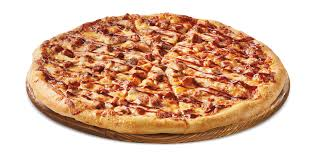
\includegraphics[scale=0.5]{pizza} 
    \caption{Pizza - sourced from https://www.cicis.com/} 
  \label{fig:pizza}
    \vspace{4ex}
  \end{minipage}%%
  \begin{minipage}[h]{0.5\linewidth}
    \centering
    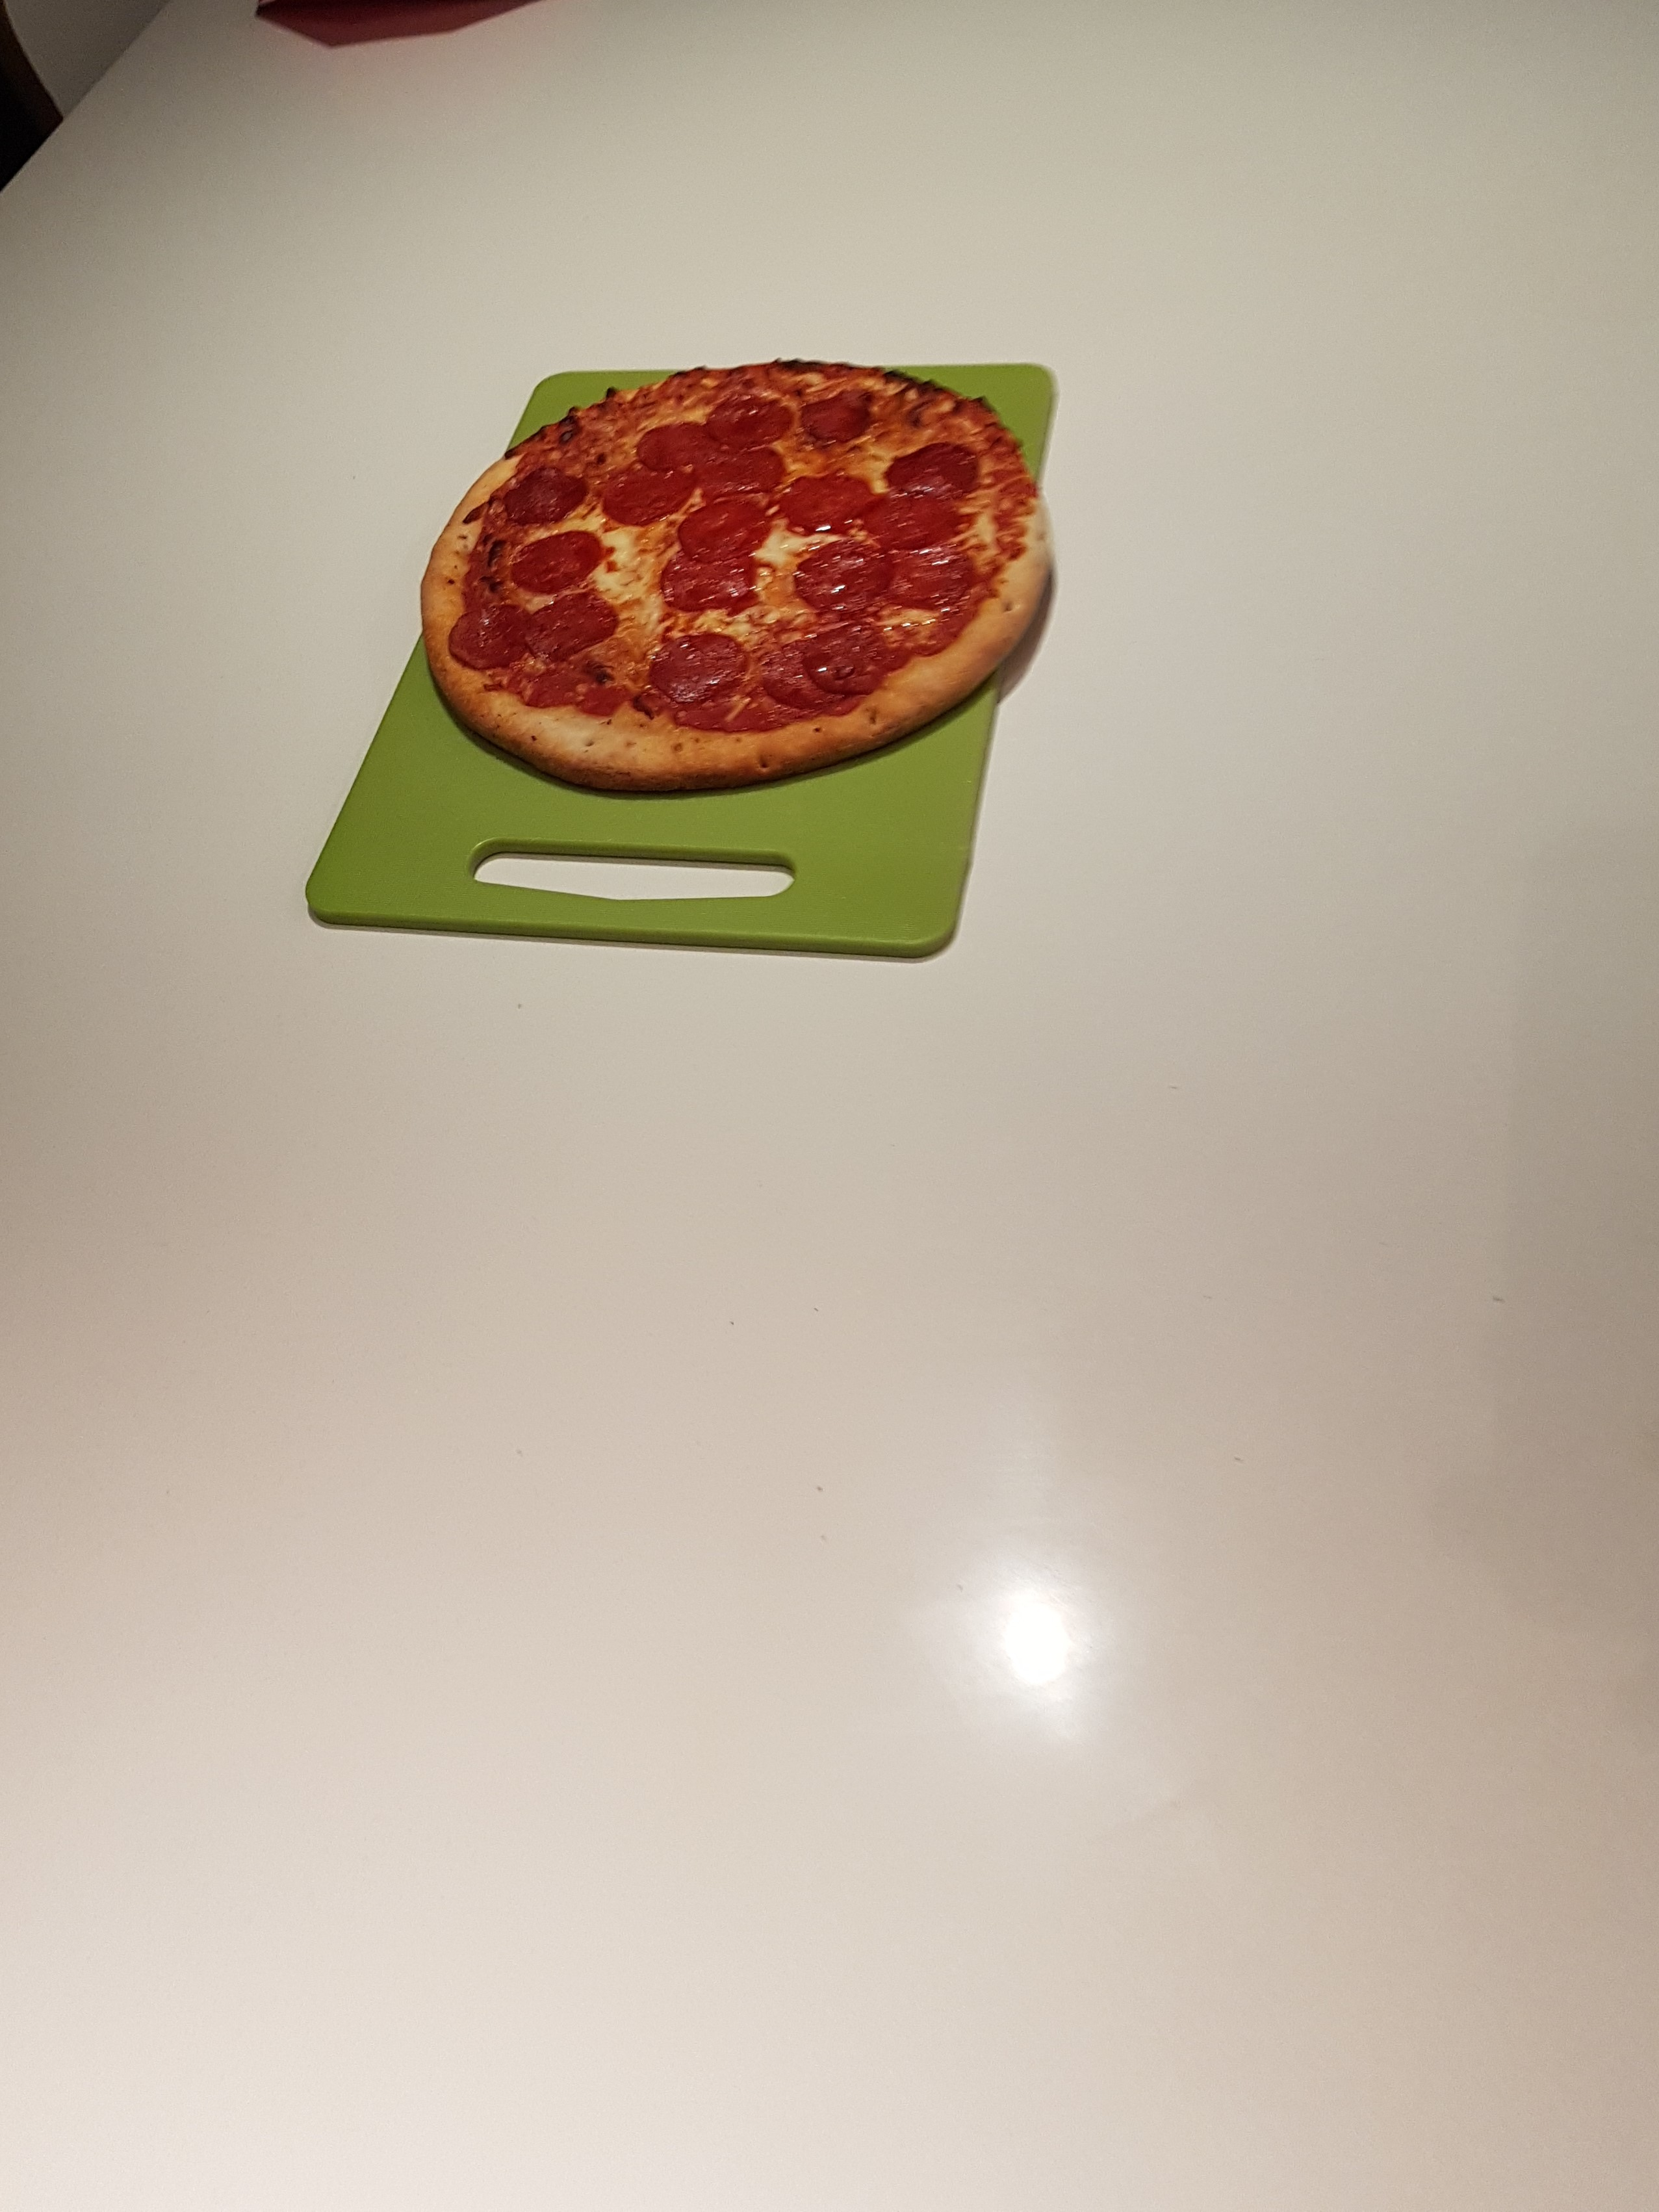
\includegraphics[scale=0.065]{pizza_unclassified} 
    \caption{Pizza not classified correctly by the model} 
  \label{fig:pizza_unclassified}
    \vspace{4ex}
  \end{minipage} 
\end{figure}

\subsection*{Analysis}
These poor results are not that surprising.
This is because we have many classes to train for, 101, and no parameter tuning has been carried out on the running of this code.
Figure \ref{fig:pizza_unclassified} was not classified correctly, this is most likely due to the fact that the pizza does not take up much of the image.



\section{Retrain with Extended Dataset}
\label{extended}
\subsection*{Overview}
For my fifth experiment, I decided to take inspiration from
\textcite{yanaiFood}, where pre-training was used training a model for food
classification. In order to achieve this, I retrained the final layer of the
Inception V3 model which was trained on the ImageNet dataset. This is called
Transfer Learning. I followed the tutorial by Google on the tensorflow website
for direction on this process \textcite{retrainInception}.

Firstly, in order to retrain the final layer of a model, a dataset must be
prepared in the correct way. I used the Food-101 dataset \textcite{food101}
which I will analyse in a later section. The dataset must be structured so that
there is a separated directory for each class with the directory name as the class
name. These directories should contain all the images for this class. 

Once this dataset has been set up correctly, a directory can be found on github
which contains the necessary files for this tutorial. When the directory has
been downloaded, the following command can be ran:
\begin{lstlisting}
python tensorflow/examples/image_retraining/retrain.py \ --image_dir
~/dataset_directory
\end{lstlisting}

The first thing that the script will do is create bottleneck files for the
images. A bottleneck is a term used to define the final layer before the output
layer. This is so that for each image, we do not have to push it through the
entire network during training \textcite{retrainInception}.

After, the bottlenecks are created, the training can be completed. The images
are split into three sub directories of training, testing and validation. By
default, these images are split into percentages of 80\%, 10\% and 10\%
respectively. The model is trained at a default of 4000 steps. 

At the final stage of the script, the model is run on a batch of test images not
yet seen and a final test accuracy is displayed. This can be seen in the Script
section below.

The command used for using this model once it is trained is:
\begin{lstlisting}
python tensorflow/examples/label_image.py --graph=/tmp/output_graph.pb
--labels=/tmp/output_labels.txt --input_layer=Mul --output_layer=final_result
--input_mean=128 --input_std=128 --image=~/image_directory
\end{lstlisting}

\subsection*{Network Architecture}
The Inception V3 model network architecture was used which consists of 22
layers.

\subsection*{Dataset}
The dataset used for this experiment is the Food-101 dataset \textcite{Food
101}. This dataset has 101 classes with 1000 images for each class.

\subsection*{Libraries}
Tensorflow and Numpy were used to run this scipt.

\subsection*{Script}
The following snippets of code are from the retrain.py script.

\begin{lstlisting}
# Add the new layer that we'll be training.
(train_step, cross_entropy, bottleneck_input, ground_truth_input,
final_tensor) = add_final_training_ops(
            len(image_lists.keys()), FLAGS.final_tensor_name,
            bottleneck_tensor,
            model_info['bottleneck_tensor_size'],
            model_info['quantize_layer'])
 
# Create the operations we need to evaluate the accuracy of our new layer.
evaluation_step, prediction = add_evaluation_step(
final_tensor, ground_truth_input)
 
# Merge all the summaries and write them out to the summaries_dir
merged = tf.summary.merge_all()
train_writer = tf.summary.FileWriter(FLAGS.summaries_dir + '/train',
                                     sess.graph)
 
validation_writer = tf.summary.FileWriter(
    FLAGS.summaries_dir + '/validation')
 
# Set up all our weights to their initial default values.
init = tf.global_variables_initializer()
sess.run(init)

\end{lstlisting}




\begin{lstlisting}
# We've completed all our training, so run a final test evaluation on
# some new images we haven't used before.
test_bottlenecks, test_ground_truth, test_filenames = (
    get_random_cached_bottlenecks(
        sess, image_lists, FLAGS.test_batch_size, 'testing',
        FLAGS.bottleneck_dir, FLAGS.image_dir, jpeg_data_tensor,
        decoded_image_tensor, resized_image_tensor, bottleneck_tensor,
        FLAGS.architecture))
test_accuracy, predictions = sess.run(
   [evaluation_step, prediction],
   feed_dict={bottleneck_input: test_bottlenecks,
        ground_truth_input: test_ground_truth})
tf.logging.info('Final test accuracy = %.1f%% (N=%d)' %
                (test_accuracy * 100, len(test_bottlenecks)))
\end{lstlisting}

\subsection*{Results}
The final test accuracy for this retrained model was 54.8\%.

For example, an image of pizza, see \ref{fig:pizza} was fed into the model with the followng results:
\begin{itemize}
    \item{pizza 0.925}
    \item{pancakes 0.008}
    \item{nachos 0.007}
    \item{beef carpaccio 0.006}
    \item{tiramisu 0.004}
\end{itemize}

\begin{figure}
     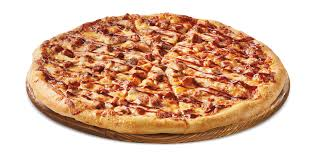
\includegraphics{pizza}
     \caption{Pizza}
     \label{fig:pizza}
\end{figure}

\subsection*{Analysis}


\section{Retrain with Parameter Tuning}
\label{parameterTuning}
\tocless\subsection{Objective}
Within the retrain.py script \parencite{retrainInception}, as mentioned in
previous experiments, there are various parameters that can be set and changed.
Various combinations of these parameters were changed to see if it would increase the
test accuracy of the model.

\begin{table}[h]
\centering
\caption{Retrain with Parameter Tuning}
\label{my-label}
\begin{tabular}{|l|p{8cm}|}
\hline
\textbf{Network Architecture} & Inception-V3           \\ \hline
\textbf{Dataset}              & Food-101+ dataset \\ \hline
\textbf{APIs and Libraries}   & TensorFlow and NumPy                                                       \\ \hline
\end{tabular}
\end{table}

\tocless\subsection{Script}
Script as seen in \ref{inception} but with some additions to calculate Top 5 accuracy as seen
in Figure \ref{lst:top5}.
Also documented is the code used to label a new image using the model (Figure \ref{lst:labelImage2}).

Figure \ref{lst:top5} takes 10 images for each class and runs each through the model.
The script then checks if the expected value is within the top 5 predictions returned from Figure \ref{lst:labelImage2}.
If it is the amount of correct top 5 predictions is incremented by one.
To calculate the Top-5 accuracy, the number of correct top-5 predictions is divided by the total number of images tested (10 images per class x number of classes) and multiplied by 100 for obtain a percentage value.


\begin{figure}[h]
\caption{Retrain Inception With Parameter Tuning Command}
\label{lst:retrainParameterCommand}
\begin{lstlisting}
python retrain_top5.py \ --image_dir
~/dataset_directory \ --how_many_training_steps 4000 \ --learning_rate 0.01 \
--testing_percentage 10 \ --validation_percentage 10
\end{lstlisting}
\end{figure}

Top 5 accuracy of the model was also calcultaed using the code below.
\begin{figure}[h]
\caption{Top-5 Accuracy Calculation}
\label{lst:top5}
\begin{lstlisting}[style=Python]
#Variables used to store a list of all classes, the amount of images tested,
# the amount of images with a top 5 accuracy and the sum of the highest probabilities
classes = list(image_lists.keys())
image_count = 0
top_5_count=0
total_of_top1_probs = 0
i = 0 
class_counter = 0

#Loops through all test images, selecting 10 images per class 
#and running them through the method in 'label_image.py'.
while(i < len(test_bottlenecks)):
  class_counter += 1
  
  if class_counter > 10:
    i = int(round((i + len(test_bottlenecks)/len(classes)) - 10))
    class_counter = 0
  else:
    image_count += 1
    results_from_classifier = label_image.runModel(test_filenames[i])
    results = results_from_classifier[0]
    probabilities = results_from_classifier[1]

    if classes[test_ground_truth[i]] in results:
      top_5_count += 1
    else:
      print("Expected:  " + classes[test_ground_truth[i]])
      for result in results:
        print("Classes: " + result)
      print("")

    total_of_top1_probs += max(probabilities)
    i = i + 1
print(str(top_5_count))
average_probabilities = total_of_top1_probs/(len(classes*10))

#Prints out the amount of test images used, the top 5 accuracy
# and the average probability of predictions.
print("Amount of test images: " + str(image_count))
print("Top 5 Accuracy: " + str((top_5_count/image_count)*100))
print("Average probability: " + str(average_probabilities))
\end{lstlisting}
\end{figure}

\begin{figure}[h]
\caption{Label Image - adapted from \parencite{retrainInception}}
\label{lst:labelImage2}
\begin{lstlisting}[style=Python]
def runModel(file_name):
  model_file = \
    "/tmp/output_graph.pb"
  label_file = "/tmp/output_labels.txt"
  input_height = 299
  input_width = 299
  input_mean = 128
  input_std = 128
  input_layer = "Mul"
  output_layer = "final_result"

  graph = load_graph(model_file)
  t = read_tensor_from_image_file(file_name,
                                  input_height=input_height,
                                  input_width=input_width,
                                  input_mean=input_mean,
                                  input_std=input_std)

  input_name = "import/" + input_layer
  output_name = "import/" + output_layer
  input_operation = graph.get_operation_by_name(input_name)
  output_operation = graph.get_operation_by_name(output_name)

  with tf.Session(graph=graph) as sess:
    results = sess.run(output_operation.outputs[0],
                      {input_operation.outputs[0]: t})
  results = np.squeeze(results)

  top_k = results.argsort()[-5:][::-1]
  labels = load_labels(label_file)
  
  setIndex = False

  top5_results = [None] * 5
  index = 0
  for i in top_k:
    top5_results[index] = labels[i]
    index += 1

  final_results = [top5_results, results]
  return final_results
\end{lstlisting}
\end{figure}

Some further parameters could be set such as:
\begin{itemize}
	\item{--flip\_left\_right}
	\item{--random\_crop}
	\item{--random\_scale}
	\item{--random\_brightness}
\end{itemize}

\begin{figure}[h]
    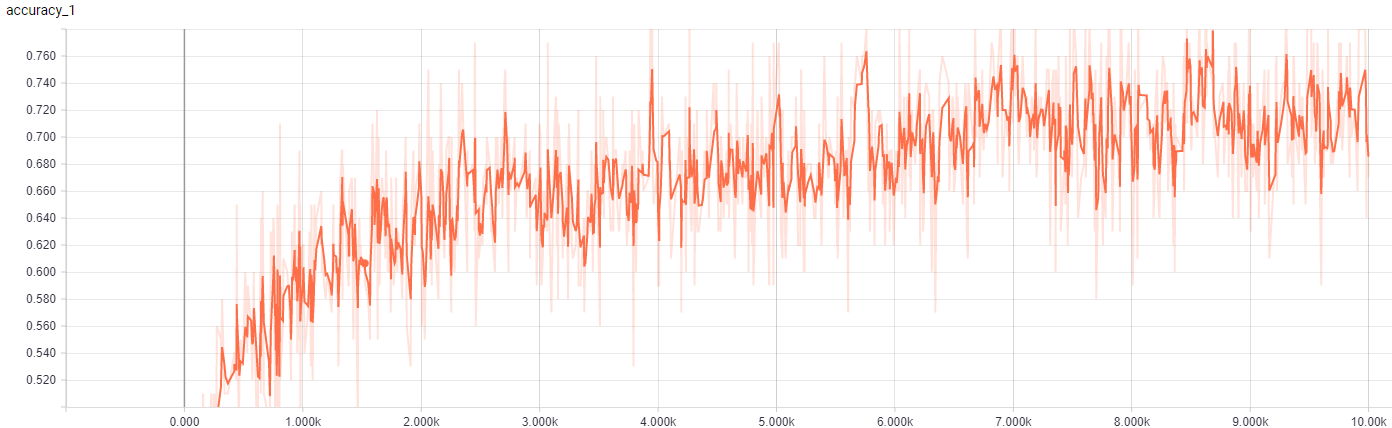
\includegraphics[scale=0.4]{model_test}
     \caption{Graph of accuracy of the test dataset during training}
     \label{fig:model_train_test}
\end{figure}

\begin{figure}[h]
    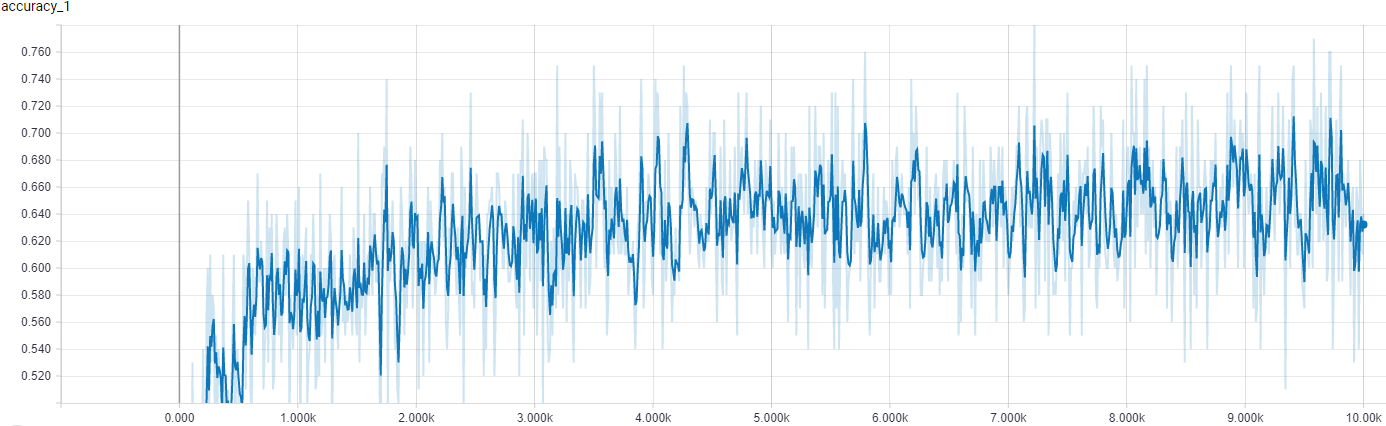
\includegraphics[scale=0.4]{model_val}
     \caption{Graph of accuracy of the validation dataset during training}
     \label{fig:model_train_val}
\end{figure}

\begin{figure}[h]
    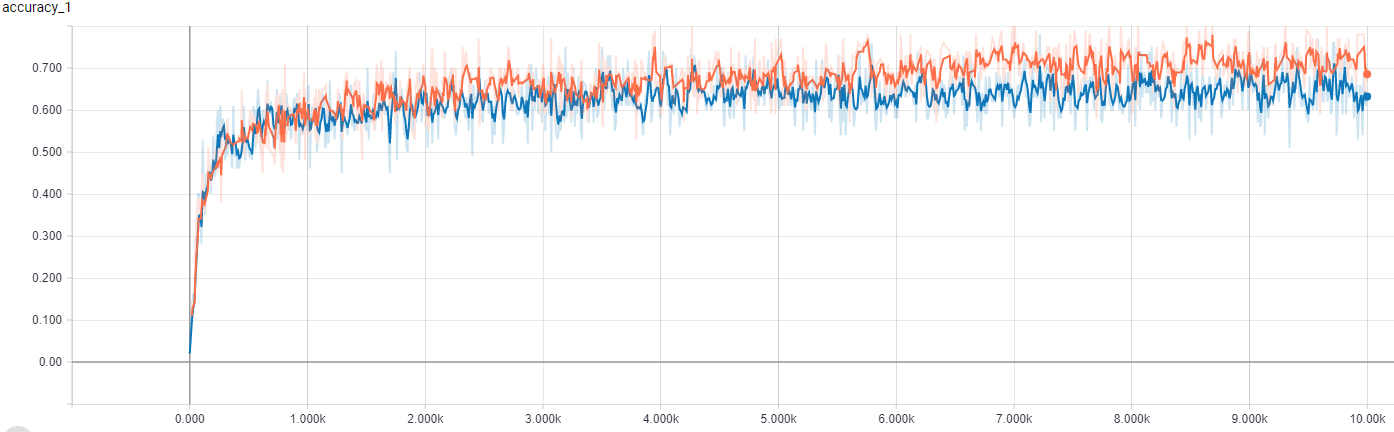
\includegraphics[scale=0.4]{test_val_accuracy}
     \caption{Comparison of accuracy}
     \label{fig:test_val_accuracy}
\end{figure}

\begin{figure}[h]
    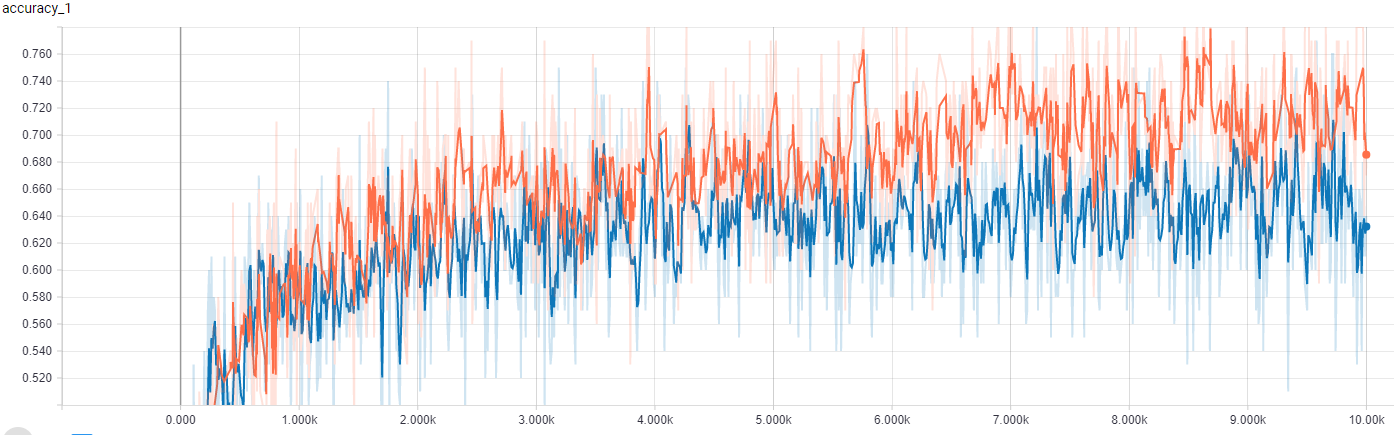
\includegraphics[scale=0.4]{test_val_accuracy_refined}
     \caption{Comparison of accuracy}
     \label{fig:test_val_accuracy_refined}
\end{figure}


\begin{table}[]
	\centering
	\caption{Comparison of parameters}
	\label{parameter_tuning_table}
	\begin{tabular}{|p{3cm}|l|l|l|l|l|}
  \hline
		\textbf{Parameter Tuning} & \textbf{Steps} & \textbf{Learning Rate} & \textbf{Test} \% & \textbf{Validation} \% &
		\textbf{Results} \\ \hline
		Configuration 1  & 8,000  & 0.01       & 10 & 10       &
		59.1\%  \\ \hline
		Configuration 2  & 8,000  & 0.10           & 10 & 10       &
		65.8\%  \\ \hline
		Configuration 3  & 10,000 & 0.10           & 10 & 10       &
		66.3\%  \\ \hline
		Configuration 4  & 12,000 & 0.10           & 10 & 10       &
		66.6\%  \\ \hline
		Configuration 5  & 10,000 & 0.20           & 10 & 10       &
		66.0\%  \\ \hline
		Configuration 6  & 10,000 & 0.10           & 15      & 15            &
		66.3\%  \\ \hline
	\end{tabular}
\end{table}

\tocless\subsection{Results}
The results of each set of parameters can be seen in Table
\ref{parameter_tuning_table}.
Using the parameters of 10,000 steps, and a learning rate of 0.1 and therefore a final test accuracy of 66.3\%, the model achieved a Top 5 accuracy of 85.96\%.
This Top-5 accuracy was calculated from 1090 images in the test dataset and the average probability of the predictions were at 0.62.
The 95\% confidence interval of the Top-1 accuracy of this model is between 57.4\% and 75.2\%.


\tocless\subsection{Analysis}
The set of parameters that seem to be the most
effective are 10,000 steps with a 0.1 learning rate. Graphs of this model can be
seen in Figures \ref{fig:model_train_val} and \ref{fig:model_train_test}. These
are based on the validation set and then the test set respectively. A side by
side comparison can also be seen in Figures \ref{fig:test_val_accuracy} and
\ref{fig:test_val_accuracy_refined} where orange is for during training and blue
for the validation set.

There were two separate factors that each increased classification accuracy of
about 5\% each. These were training steps and learning rate.

Training steps are related to the number of images so before, when the training
steps were at 4,000, not all of the training images were being used. As the steps were increased
twofold we saw a 3.8\% increase in accuracy.

Another parameter that increased accuracy significantly was learning rate. The
default learning rate is 0.01 which was increased to 0.1. This resulted in an
increase of 6.7\%. This is most likely since we are only
looking at the last layer, we can afford to change the weights more
significantly.

The Top 5 accuracy of the model was quite good but it was not run on the same number of images as the final test accuracy.
This is beacuse TensorFlow does not have an API for calculating Top 5 accuracy.
As a result, it had to be calculated manually and this is very time intensive.
The average probability of 0.62 is also quite close to the overall Top 1 accuracy which may imply some correlation between the two but this is merely speculation.

\afterpage{\clearpage}


\section{MobileNet}
\label{mobilenet}
\tocless\subsection{Objective}
Since the end goal for this project is to have a smartphone
application that a user can use to keep track of their calorie measurement,
there are a couple of options in how to achieve this. Firstly, an image can be
taken on the phone and sent to a server to run a classification algorithm.
Secondly, a model can be stored on the phone for computation. Transfer learning was once again used but on a different, smaller architecture called MobileNet \parencite{mobilenet}.

\begin{table}[h]
\centering
\caption{MobileNet}
\label{my-label}
\begin{tabular}{|l|p{8cm}|}
\hline
\textbf{Network Architecture} & MobileNet           \\ \hline
\textbf{Dataset}              & Food-101+ dataset \\ \hline
\textbf{APIs and Libraries}   & TensorFlow and NumPy                                                       \\ \hline
\end{tabular}
\end{table}

\tocless\subsection{Script}
The retrain.py script \parencite{retrainInception} was used, with a different
command parameter.

\begin{lstlisting}[style=Command]
python tensorflow/examples/image_retraining/retrain.py \ --image_dir
~/dataset_directory \ --architecture mobilenet_1.0_224 \
--how_many_training_steps 10000 \ --learning_rate 0.1
\end{lstlisting}

\tocless\subsection{Results}
The final test accuracy of this model came to 50.2\%.

\tocless\subsection{Analysis}
There was a decrease of 16.1\% in this model to the highest accuracy from
\ref{mobilenet}. This is due to the smaller architecture which is aimed to be faster
and smaller with an expected decrease in accuracy.


\section{Food 101 subset}
\label{subset}
\subsection*{Objective}
In many of the papers that have been researched where food image classification was carried out, they attempted to classify a lot less than 108 food types as has been the case for experiments previously shown.
\parencite{novelSVM} used 12 classes, \parencite{pouladzadeh2014measuring} had 15, \parencite{LSL_2015} attempted to classify 11 classes of food, 20 classes were used in \parencite{chen2010toward} and \parencite{snap} predicted 15 classes.
Due to the lower number of classes in these papers, it was decided to retrain inception on a subset of the food-101 extended dataset to benchmark results.
13 classes were selected from food-101 for training.

\subsection*{Network Architecture}
Retrained Inception model.

\subsection*{Dataset}
A subset of the Food 101 dataset was used for this experiment \parencite{food101}.

\subsection*{Results}
A Final test Accuracy of 92.6\% was recorded for this experiment which performs quite high in comparison to the data in Table \ref{classes_accuracy}.
A Top 5 accuracy of 100\% was calculated with an average prediction probability of 0.89 using 130 images.
This was calculated using the script defined in \ref{parameterTuning}.

\begin{table}[]
\centering
\caption{Accuracy of other studies}
\label{classes_accuracy}
\begin{tabular}{|l|l|l|}
\hline
\textbf{Reference}                       & \textbf{Classes} & \textbf{Accuracy}      \\ \hline
Novel SVM                       & 12      & 92.6\%        \\ \hline
Measuring Calorie and Nutrition & 15      & 90.4\%       \\ \hline
Large Scale Learning            & 11      & 78.0\%          \\ \hline
Toward Dietary Assessment       & 20      & 91.7\% \\ \hline
Snap-n-eat                      & 15      & 85.0\%         \\ \hline
\end{tabular}
\end{table}

\subsection*{Analysis}
It would make sense the accuracy of our model would increase when the number of classes are reduced as the margin of error is decreased.
The Top 5 accuracy of the model was very successful.
There were only 10 images per class tested though, totaling at 130 images so if the number of images increased, this accuracy would probably decrease slightly.
If the code is run again, the same results cannot even be replicated for sure.
On another run of this code a Top 5 accuracy of 96\% was recorded.
While this is still a very good accuracy, it does not compare to the first run of the script.

\chapter{Analysing the Trained Model}

\section{Sliding Window}
\label{slidingWindow}
\subsection*{Overview}
In the preious experiments, I have looked at the one-shot approach to food image
classification. That is, the model will give a prediction of the most likely
food item in that image. This is a problem when there are multiple food in an
image, see \ref{fig:fruit}. There are a few options to combat this problem. Firstly, I could detect
objects in the image, segment the image according to these objects and then run
each segment through the model. A simple approach to this would be to segment
the image into a number of sections and then run each section through the model.
In order to follow the latter approach, I used a sliding window approach. This
sliding window would move across the image and classify the segment of the image
in the window. I had three options for window sliding shape as defined by a
command line argument.

\begin{lstlisting}
python sliding_window.py --image=~/image_dir --window_shape grid
\end{lstlisting}

There are three options for window shape:
\begin{itemize}
	\item{Grid based window as per \ref{fig:fruitGrid}}
	\item{Row based window as per \ref{fig:fruitRow}}
	\item{Column based window as per \ref{fig:fruitColumn}}
\end{itemize}

\begin{figure}
    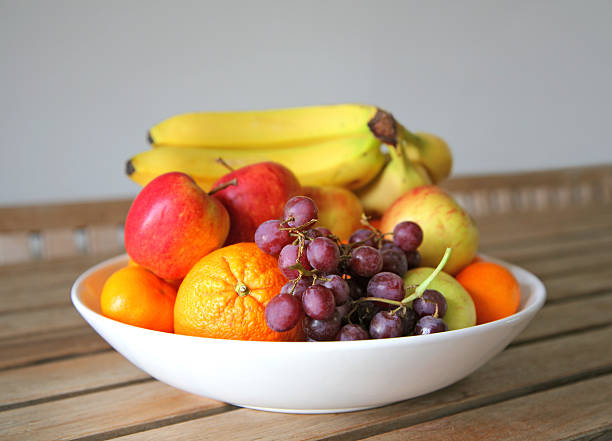
\includegraphics[scale=0.5]{fruit}
    \caption{Bowl of fruit}
    \label{fig:fruit}
\end{figure}

\begin{figure}
    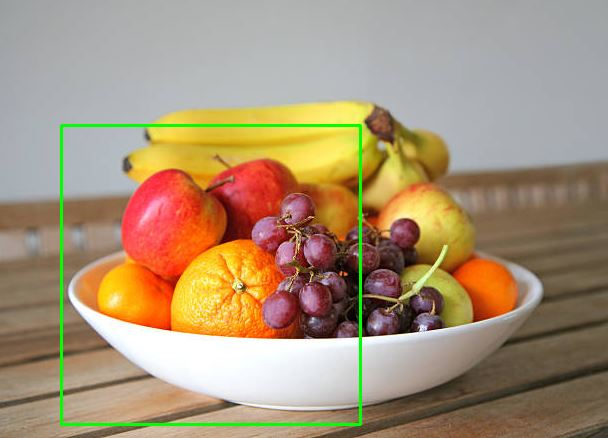
\includegraphics[scale=0.5]{fruitGrid}
	\caption{Grid based window}
    \label{fig:fruitGrid}
\end{figure}

\begin{figure}
    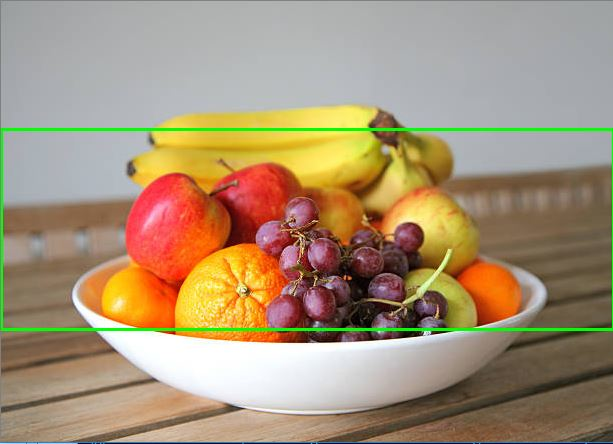
\includegraphics[scale=0.5]{fruitRow}
    \caption{Row based window}
    \label{fig:fruitRow}
\end{figure}

\begin{figure}
    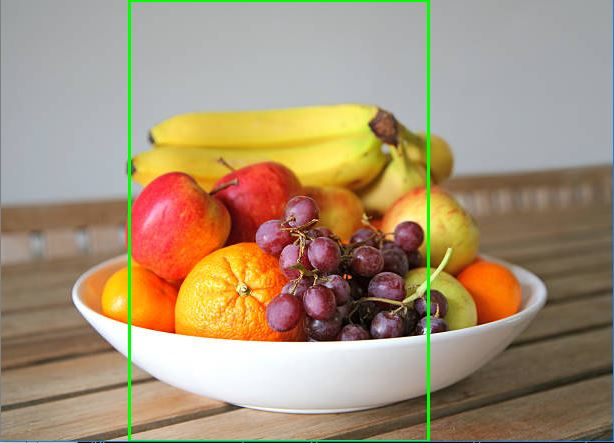
\includegraphics[scale=0.5]{fruitColumn}
    \caption{Column Based Window}
    \label{fig:fruitColumn}
\end{figure}

\begin{figure}
    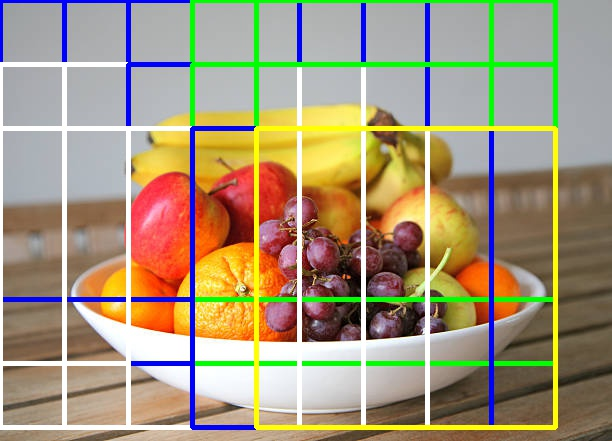
\includegraphics[scale=0.5]{fruitCO}
    \caption{Fruit with Color Overlay}
    \label{fig:fruitOverlay}
\end{figure}

\subsection*{Libraries}
For this experiment Tensorflow provided the classification of each segment while
also helping with resizing along with Numpy. OpenCv was used to implement the
sliding window as per \textcite{slidingWindowTut}

\subsection*{Script}
There were four main elements to the script. Firstly, extracting a window to be
classified. Secondly, resizing the image to be compatible with the Tensorflow
model. Thirdly, running the window through the Tensorflow model and finally
saving a new image with a coloured overlay of classifications.

\subsubsection*{Extracting the window from the image}
\begin{lstlisting}
# loop over the image pyramid
for resized in pyramid(image, scale=1.5):
		# loop over the sliding window for each layer of the pyramid
		for (x, y, window) in sliding_window(resized, stepSize=32, windowSize=(winW, winH)):
			# if the window does not meet our desired window size, ignore it
				if window.shape[0] != winH or window.shape[1] !=winW:
					continue
\end{lstlisting}


\begin{lstlisting}
def sliding_window(image, stepSize, windowSize):
	# slide a window across the image
	for y in xrange(0, image.shape[0], stepSize):
		for x in xrange(0, image.shape[1], stepSize):
			# yield the current window
			yield (x, y, image[y:y + windowSize[1], x:x + windowSize[0]])
\end{lstlisting}

\subsubsection*{Resizing the window}
\begin{lstlisting}
window = cv2.resize(window, (299, 299))
\end{lstlisting}

\begin{lstlisting}
resized_image = tf.reshape(image, [1, input_height, input_width, 3])
resized = tf.image.resize_area(resized_image, [input_height, input_width])
normalized = tf.divide(tf.subtract(resized, [input_mean]), [input_std])
\end{lstlisting}

\subsubsection*{Running the Tensorflow model}
\begin{lstlisting}
with tf.Session() as sess:
	numpy_image = sess.run(normalized)

with tf.Session(graph=graph) as sess:
    results = sess.run(output_operation.outputs[0],
                      {input_operation.outputs[0]: numpy_image})
	probabilities = np.squeeze(results)
\end{lstlisting}

\subsubsection*{Saving the image with colour overlay}
As seen in Figure \ref{fig:fruitOverlay}, each square represents a window and
each colour is for a different classification. Blue is for an apple, yellow for
banana, green for grape, white for orange and black if an unexpected prediction
is made.

\begin{lstlisting}
cv2.rectangle(display_image, (x, y), (x + winW, y + winH), colour_dict.get(top1,
(0,0,0)), 4)
\end{lstlisting}

\subsection*{Results}
\subsubsection*{Grid based window}
The grid based window resulted in fifteen separate classification. As seen in
\ref{fig:fruit}, there are multiple fruits in the image. Of these fruits, our
model is trained on four, apple, banana, orange and grapes. This method
classified all four to Top-1 accuracy at least once each. This method took 42.8
seconds to run.

\begin{table}[]
	\centering
	\caption{My caption}
	\label{my-label}
	\begin{tabular}{ll}
		Food type & No. of Top-1 Classifications \\
		Apple     & 5                      \\
		Banana    & 1                      \\
		Grape     & 4                      \\
		Orange    & 5                     
	\end{tabular}
\end{table}

\begin{table}[]
	\centering
	\caption{My caption}
	\label{rowWindowTable}
	\begin{tabular}{ll}
		Food type & No. of Top-1 Classifications \\
		Apple     & 1                      \\
		Banana    & 0                      \\
		Grape     & 0                      \\
		Orange    & 0                      \\
		Other     & 3                     
	\end{tabular}
\end{table}

\begin{table}[]
	\centering
	\caption{My caption}
	\label{colWindowTable}
	\begin{tabular}{ll}
		Food type & No. of Top-1 Classifications \\
		Apple     & 3                      \\
		Banana    & 1                      \\
		Grape     & 0                      \\
		Orange    & 0                      \\
		Other     & 1                     
	\end{tabular}
\end{table}

\subsubsection*{Row based window}
The row based method resulted in four predictions as follows in
\ref{rowWindowTable}. Out of these four predictions, only one classified a known
fruit at Top-1 accuracy, an apple. An apple was also predicted to Top-5 accuracy
in another instance. The runtime of this method was 16.1 seconds.

\subsubsection*{Column based window}
The column based window approach had five total predictions and ran for a total
of 13 seconds. As seen in \ref{colWindowTable}, two out of four known fruits
were classified to a Top-1 accuracy with all other fruits predicted to Top-5
accuracy. Only one Top-1 prediction did not contain a correct fruit.

\subsection*{Empirical Analysis}
These results are very interesting because while a banana was only predicted to
Top-1 accuracy once in grid based, once in column based and zero times in row
based, if the whole image is ran through the model, a banana is at the Top-1 accuracy.


























\section{Recursive Refinement}
\label{RR}
\tocless\subsection{Objective}
After the sliding window code was run on Figure \ref{fig:fruit} in \ref{slidingWindow},
it was observed that a sliding window was predicting grapes correctly in
regions that contained a bunch of grapes. Since it would make sense that the
model would be able detect an individual grape, it was decided that
recursive refinement would be ran on a window that contained a grape. Due to the model
requiring a 299 x 299 image size, the window could only be refined once as
very small segments could not be resized up to 299 x 299. A window of 70 x 70 size was used.

\tocless\subsection{Script}
As you would think with recursive refinement, a recursive function would be used,
but this was unnecessary due to image size restrictions. Instead, a
conditional for loop was added to the existing code to break a window down further i.e. perform a sliding window approach on a window.
This can be seen in Figure \ref{lst:rrCode}.

\begin{figure}[h]
\caption{Recursive Refinement Code}
\label{lst:rrCode}
\begin{lstlisting}[style=Python]
if top1 == "grape" and window_shape == "grid" and rr_grape:
			for (x_grape, y_grape, grape_window) in sliding_window(window_resized, stepSize=64, windowSize=(70, 70)):
				#reshape to square
				grape_window_resized = cv2.resize(grape_window, (299, 299))
				top1_grape = subSample.classify(grape_window_resized, window_shape)
				if top1_grape == "grape":
					cv2.rectangle(display_image, (x_grape + x, y_grape + y), (x_grape + x + 70, y_grape + y + 70), colour_dict.get(top1, (0,0,0)), 4)
					#cv2.imshow("Window", grape_window_resized)
					cv2.waitKey(1)
time.sleep(0.025)
\end{lstlisting}
\end{figure}

\begin{figure}[h]
\centering
    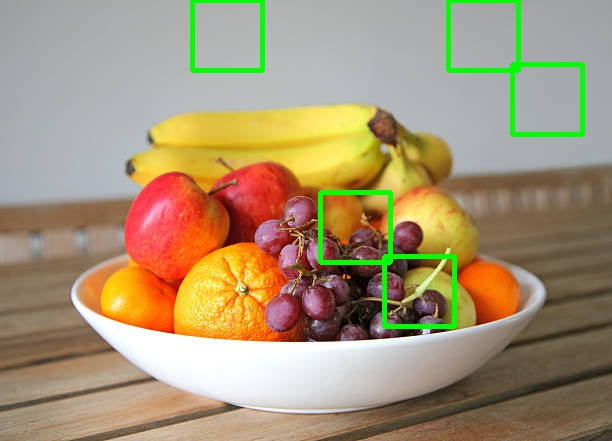
\includegraphics[scale=0.4]{fruit_rr}
      \caption{Recursive refinement 1}
      \label{fig:rr1}
\end{figure}

\tocless\subsection{Results}
Some very similar results were recorded on three separate images. Two new images are seen
here which we will explore in future experiments. In all three images, while the script
is calculating some expected predictions, grapes are being classified in locations
that have nothing resembling a grape. These can be viewed in Figures
\ref{fig:rr1}, \ref{fig:rr2} and \ref{fig:rr3}.

\tocless\subsection{Analysis}
The instances where false positives were recorded may indicate issues with the recursive refinement approach as every window must be classified and it is possible that this just happens to be a grape in some instances.
Further analysis to why this may be occurring is outlined in the section \ref{rrAnalyse}.

\begin{figure}
\centering
    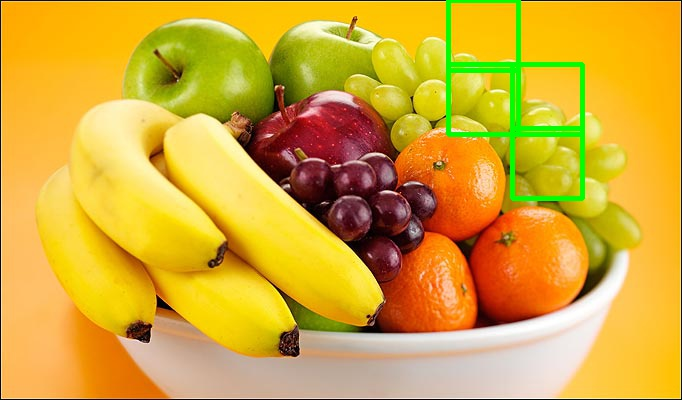
\includegraphics[scale=0.2]{newfruit_rr_grid}
      \caption{Recursive refinement 2 - sourced from http://www.travispta.org/}
      \label{fig:rr2}
\end{figure}

\begin{figure}
\centering
    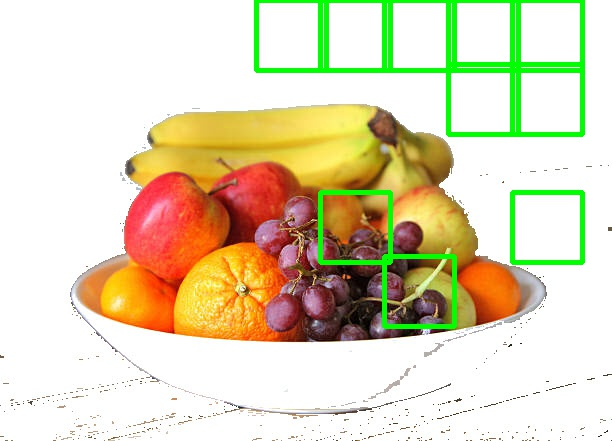
\includegraphics[scale=0.3]{processed_image}
      \caption{Recursive refinement 3}
      \label{fig:rr3}
\end{figure}



\section{Impact of Backround}
\label{background}
\tocless\subsection{Objective}
As we can see in section \ref{slidingWindow}, using sliding windows to classify many sections
of an image, there were some cases where some unexpected predictions were made.
Due to this, the decision was made to analyse the effect the background of the
image on its classification. The sliding window code was then ran on a new
image. This new image was the same fruit bowl as used previously but the
background was filled in as white as per Figure \ref{fig:filledFruit}.

\begin{figure}[h]
\centering
    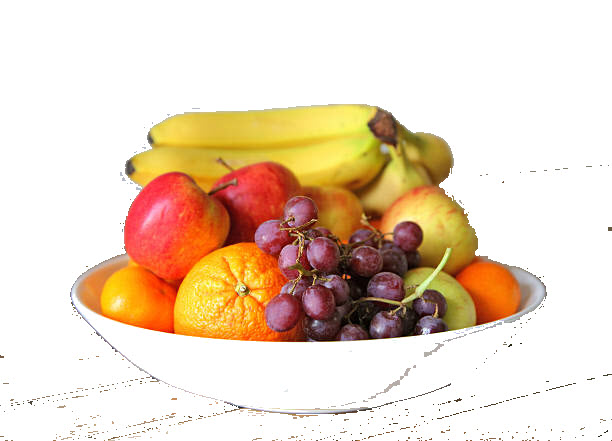
\includegraphics[scale=0.75]{fruitFillBg}
    \caption{Bowl of fruit with background removed}
    \label{fig:filledFruit}
\end{figure}

\begin{table}[h]
    \centering
    \caption{Comparison of fruit image sliding window results with and without
    background}
    \label{comparisionFruitTable}
    \begin{tabular}{|l|l|l|l|p{1.25cm}|p{1.25cm}|p{2cm}|}
    \hline
        \textbf{Food type} & \textbf{Grid} & \textbf{Row} & \textbf{Column} & \textbf{White Grid} & \textbf{White Row} & \textbf{White Column} \\ \hline
        Apple     & 5    & 1   & 3      & 10          & 0          & 4
        \\ \hline
        Banana    & 1    & 0   & 1      & 0           & 0          & 0
        \\ \hline
        Grape     & 4    & 0   & 0      & 1           & 0          & 1
        \\ \hline
        Orange    & 5    & 0   & 0      & 3           & 0          & 0
        \\ \hline
        Other     & 0    & 3   & 1      & 1           & 4          & 0  \\ \hline           
    \end{tabular}
\end{table}

\tocless\subsection{Results}
\tocless\subsubsection{Grid}
For grid-based sliding window approach, the results turned out to be less
successful than with the background. In this experiment, fourteen out of fifteen
of top-1 classification were of an expected food type rather than fifteen out of
fifteen with the background present. We expected the food types of apple,
orange, grape and banana to appear in this image but while a banana was detected
to a top-5 accuracy on a few occasions it was never predicted to a top-1
accuracy. The contrast between the image results can be seen in Table
\ref{comparisionFruitTable}.

\tocless\subsubsection{Row}
The row-based sliding window again had worse result than its counterpart, with
zero out of four correct classifications as opposed to one. In this case, an
orange appeared at top-5 accuracy once. The most common prediction was ice-cream
which appeared at top-1 accuracy in three out of four instances.

\tocless\subsubsection{Column}
In contrast to our previous two methods of sliding window, this method
outperformed its counterpart with correct predictions of all five windows while
before we only had four out of five. In this experiment, an apple was predicted
four times and a grape once, with all correct fruits appearing to top-5
accuracy.

\tocless\subsection{Analysis}
Surprisingly, removing the background of the image reduced the prediction
accuracy.
Many white foods were classified instead which makes sense due
the impact of colour expected.


\section{Alternative Test Image}
\label{alternative}
\begin{figure}
    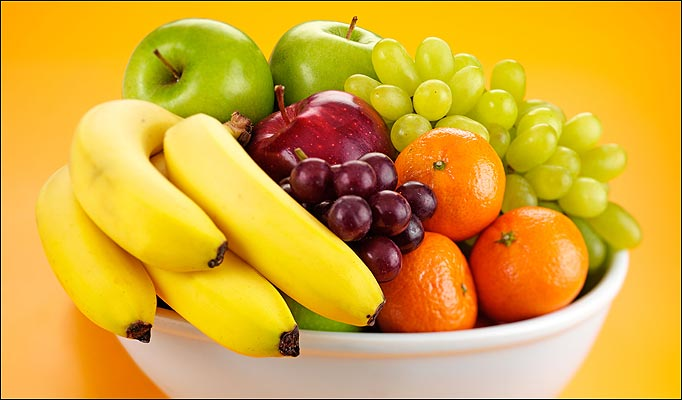
\includegraphics[scale=0.5]{fruitbowl2}
    \caption{Alternative Bowl of fruit}
    \label{fig:newFruit}
\end{figure}

\begin{table}[]
    \centering
    \caption{Comparison of fruit bowl images}
    \label{newFruitTable}
    \begin{tabular}{|l|l|l|l|l|l|l|}
    \hline
        \textbf{Food type} & \textbf{Grid} & \textbf{Row} & \textbf{Column} & \textbf{New Grid} & \textbf{New Row} & \textbf{New Column} \\ \hline
        Apple     & 5    & 1   & 3      & 4        & 1       & 0          \\ \hline
        Banana    & 1    & 0   & 1      & 5        & 0       & 5          \\ \hline
        Grape     & 4    & 0   & 0      & 2        & 1       & 0          \\ \hline
        Orange    & 5    & 0   & 0      & 0        & 0       & 0          \\ \hline
        Other     & 0    & 3   & 1      & 1        & 2       & 1         \\ \hline
    \end{tabular}
\end{table}

\subsection*{Overview}
In our previous sliding window oriented experiments, we had only used a
single image. In order to see whether this image had biases unknown
to us, another fruit bowl image had to be tested. This image was selected as
fruit took up a larger portion of the image as seen in Figure \ref{fig:newFruit}.

\subsection*{Results}
\subsubsection*{Grid}
The performance of this experiment was slightly worse than with the previously
used image. When the grid based sliding window was executed on Figure
\ref{fig:newFruit}, fourteen out of fifteen predictions had an expected value.
Out of the fourteen predictions orange was not predicted to top-1 accuracy at
all. This can be seen, in comparison to previously used image, in Table
\ref{newFruitTable}.

\subsubsection*{Row}
In the column based window for the new fruit image, the results were not very
successful as has been the trend for most row based classification. Two out of
four predictions had an expected value at top-1 accuracy.

\subsubsection*{Column}
The column based approach had a similar result to its counterpart in that only
one of its predictions was unexpected. Although, due  to the size of the new
image, another column was created and thus has a better overall accuracy.

\subsection*{Empirical Analysis}
A possible reason that an orange was not classified in any of these images is
because in Figure \ref{fig:newFruit}, a more mandarin food is displayed.


\section{Scaling Down Images}
\label{scale}
\begin{figure}
    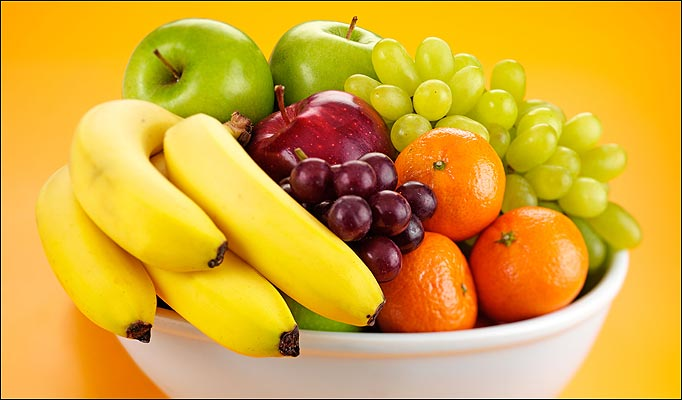
\includegraphics[scale=0.5]{fruitbowl2}
    \caption{Alternative Bowl of fruit}
    \label{fig:newFruit}
\end{figure}

\subsection*{Overview}
In our three previous sliding window oriented experiments, we had only used a
single image. In order to see whether this image had biases unknown
to us, I decided to use another fruit bowl image. This image was selected as
fruit took up a larger portion of the image as seen in Figure \ref{fig:newFruit}

\subsection*{Results}
\subsubsection*{Grid}
\subsubsection*{Row}
\subsubsection*{Column}

\subsection*{Analysis}


\section{Effect of Colour}
\label{colour}
\tocless\subsection{Objective}
As seen in the last experiment, it is possible that colour plays a significant part in the overall classification of some food types, along with shape and texture. Due to this, what would happen if colour was removed from the image? The three images, Figure \ref{fig:bananaPreRes}, Figure \ref{fig:apple_piePreRes} and Figure \ref{fig:pizzaPreRes}, were all converted to greyscale to test this and the resulting images can be seen in Figure \ref{fig:bananaGrey}, Figure \ref{fig:applePieGrey} and Figure \ref{fig:pizzaGrey}. Each of these images were ran through the model before and after converting to greyscale and the results were recorded.

\begin{figure}[h]
	\centering
    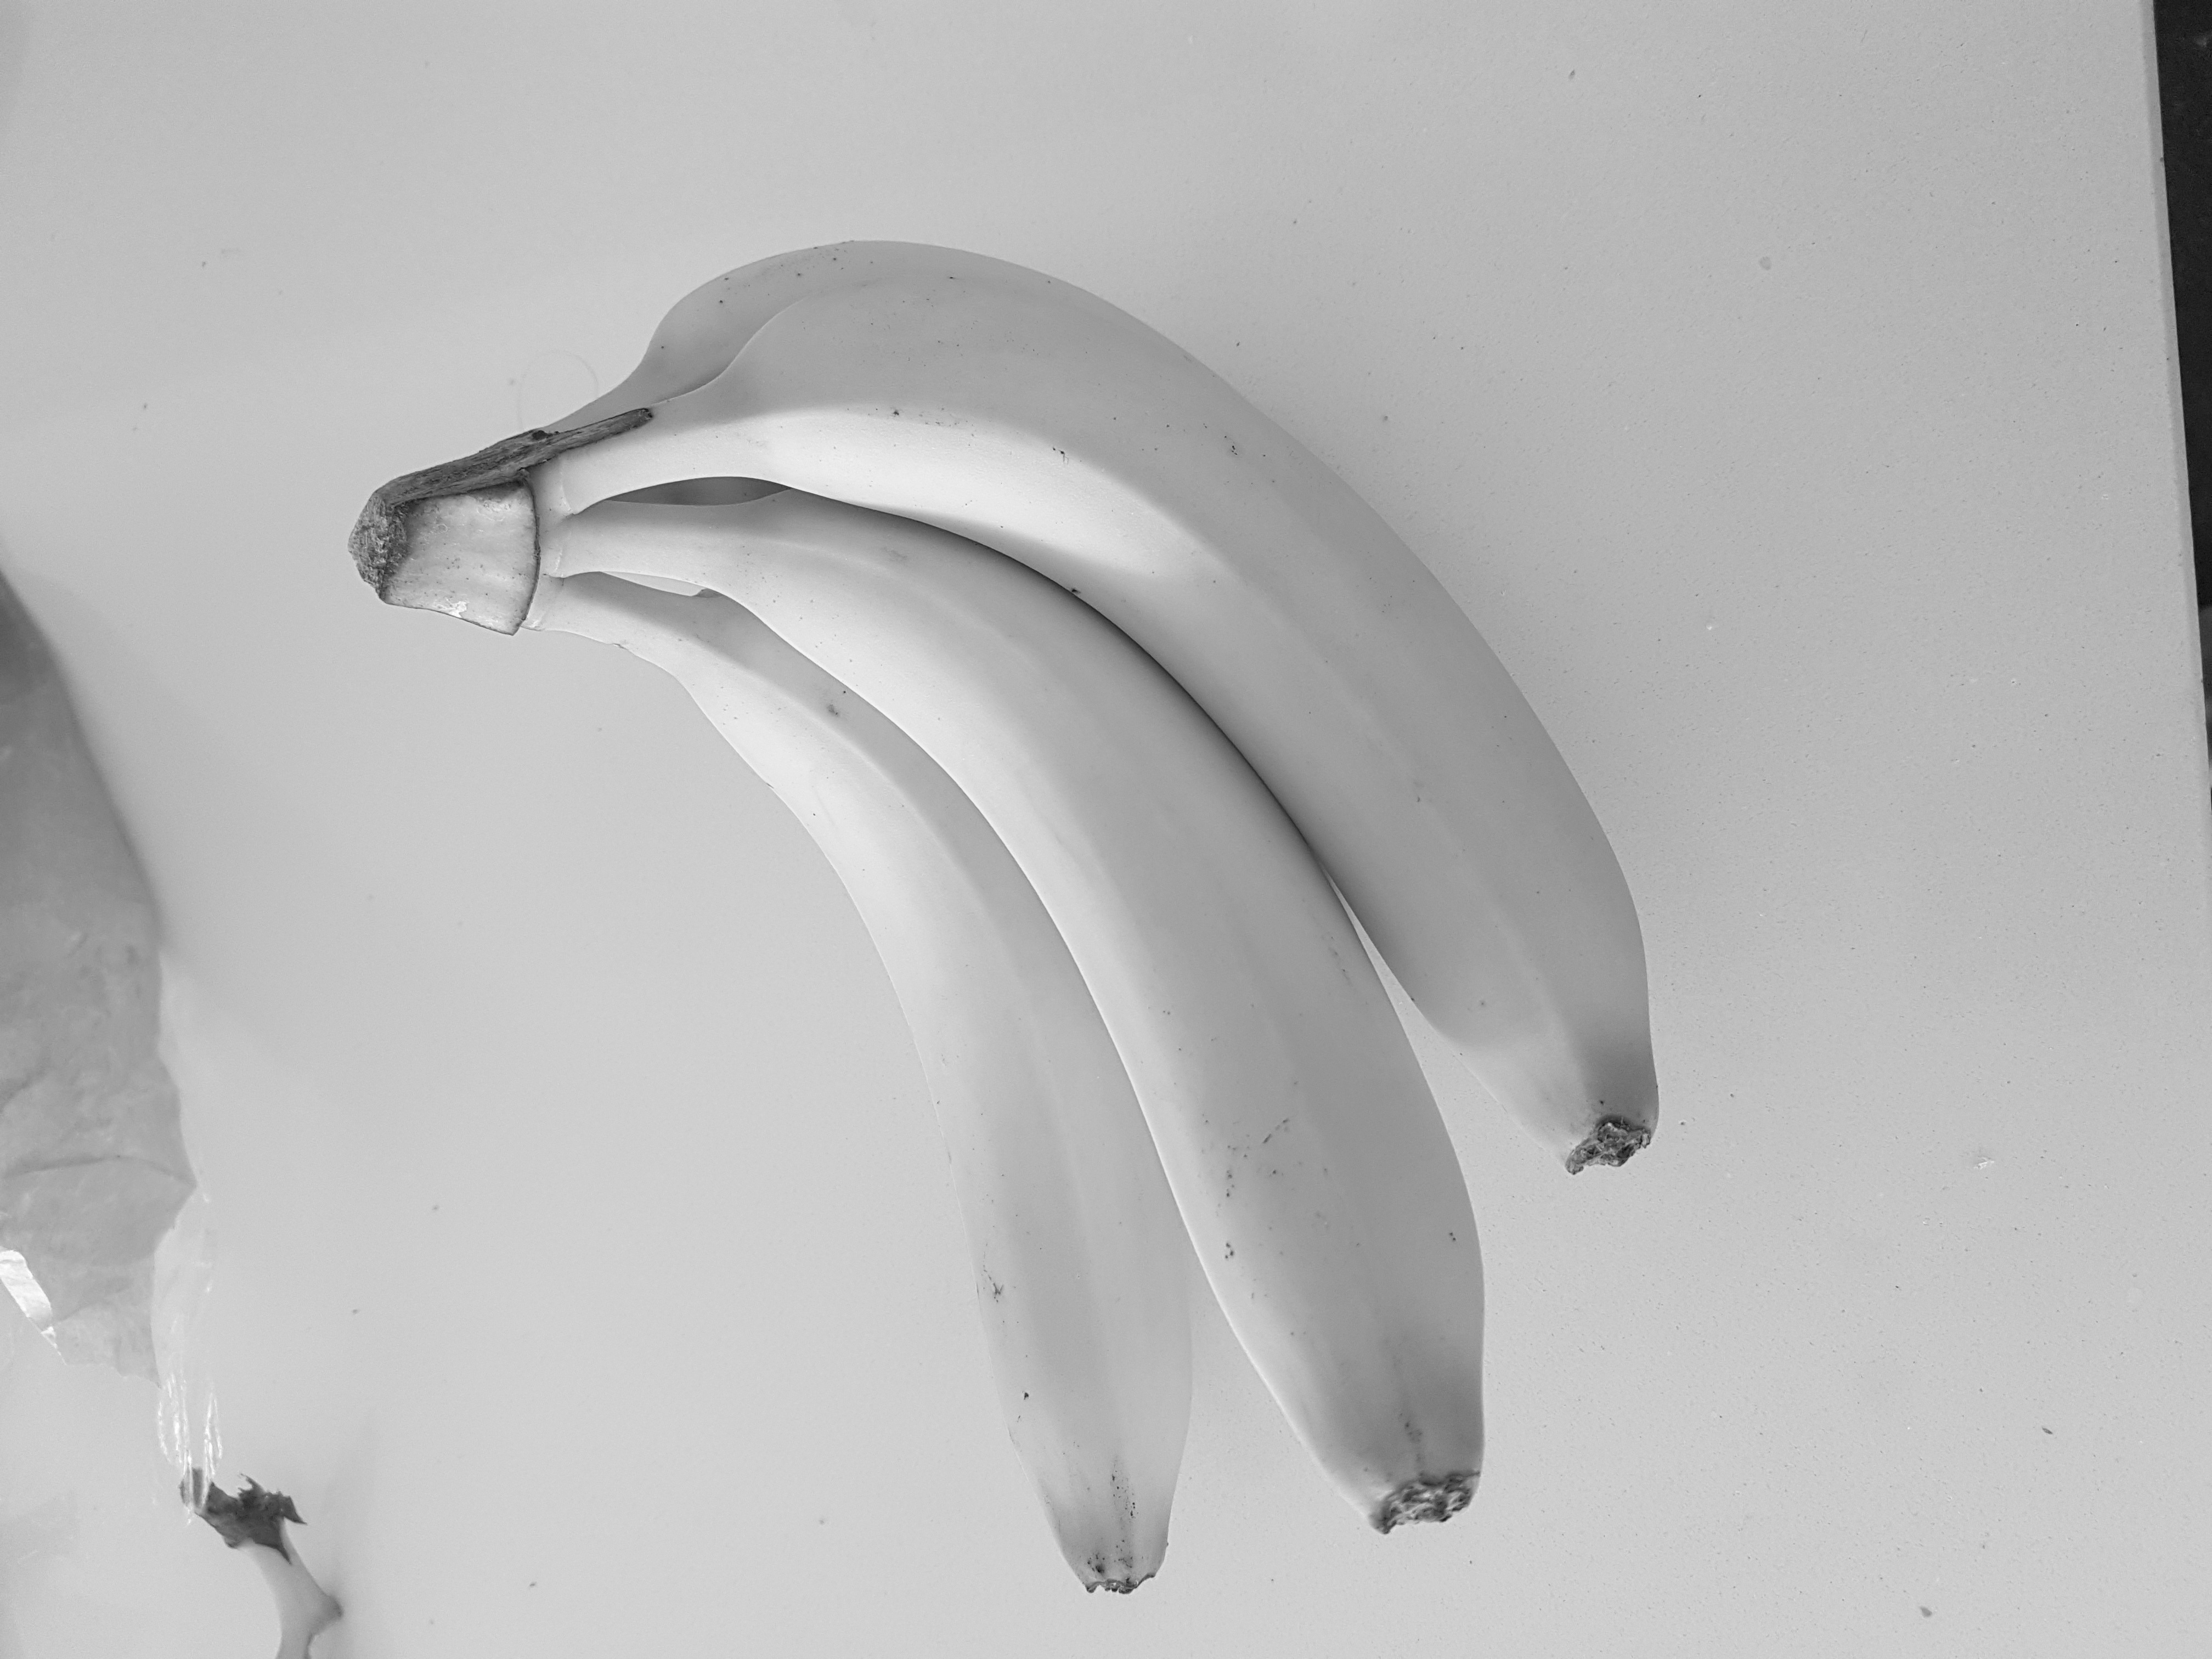
\includegraphics[scale=0.05]{banana_grey}
    \caption{Banana Image Greyscale}
    \label{fig:bananaGrey}
\end{figure}

\begin{figure}[h]
	\centering
    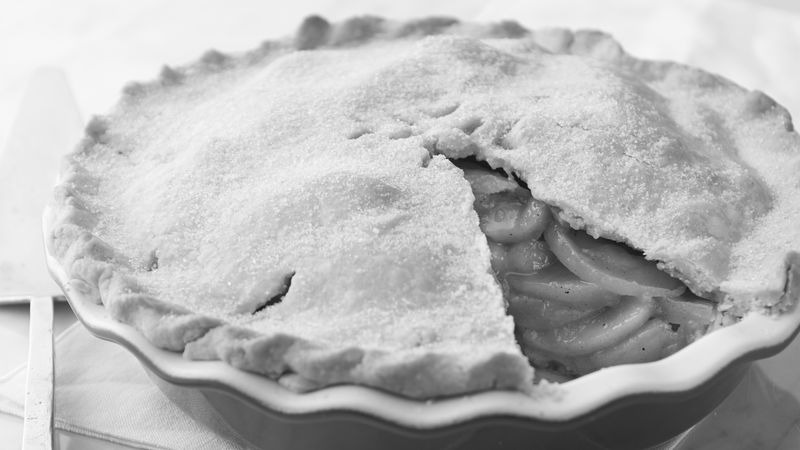
\includegraphics[scale=0.25]{pie_grey}
    \caption{Apple Pie Image Greyscale}
    \label{fig:applePieGrey}
\end{figure}

\begin{figure}[h]
	\centering
    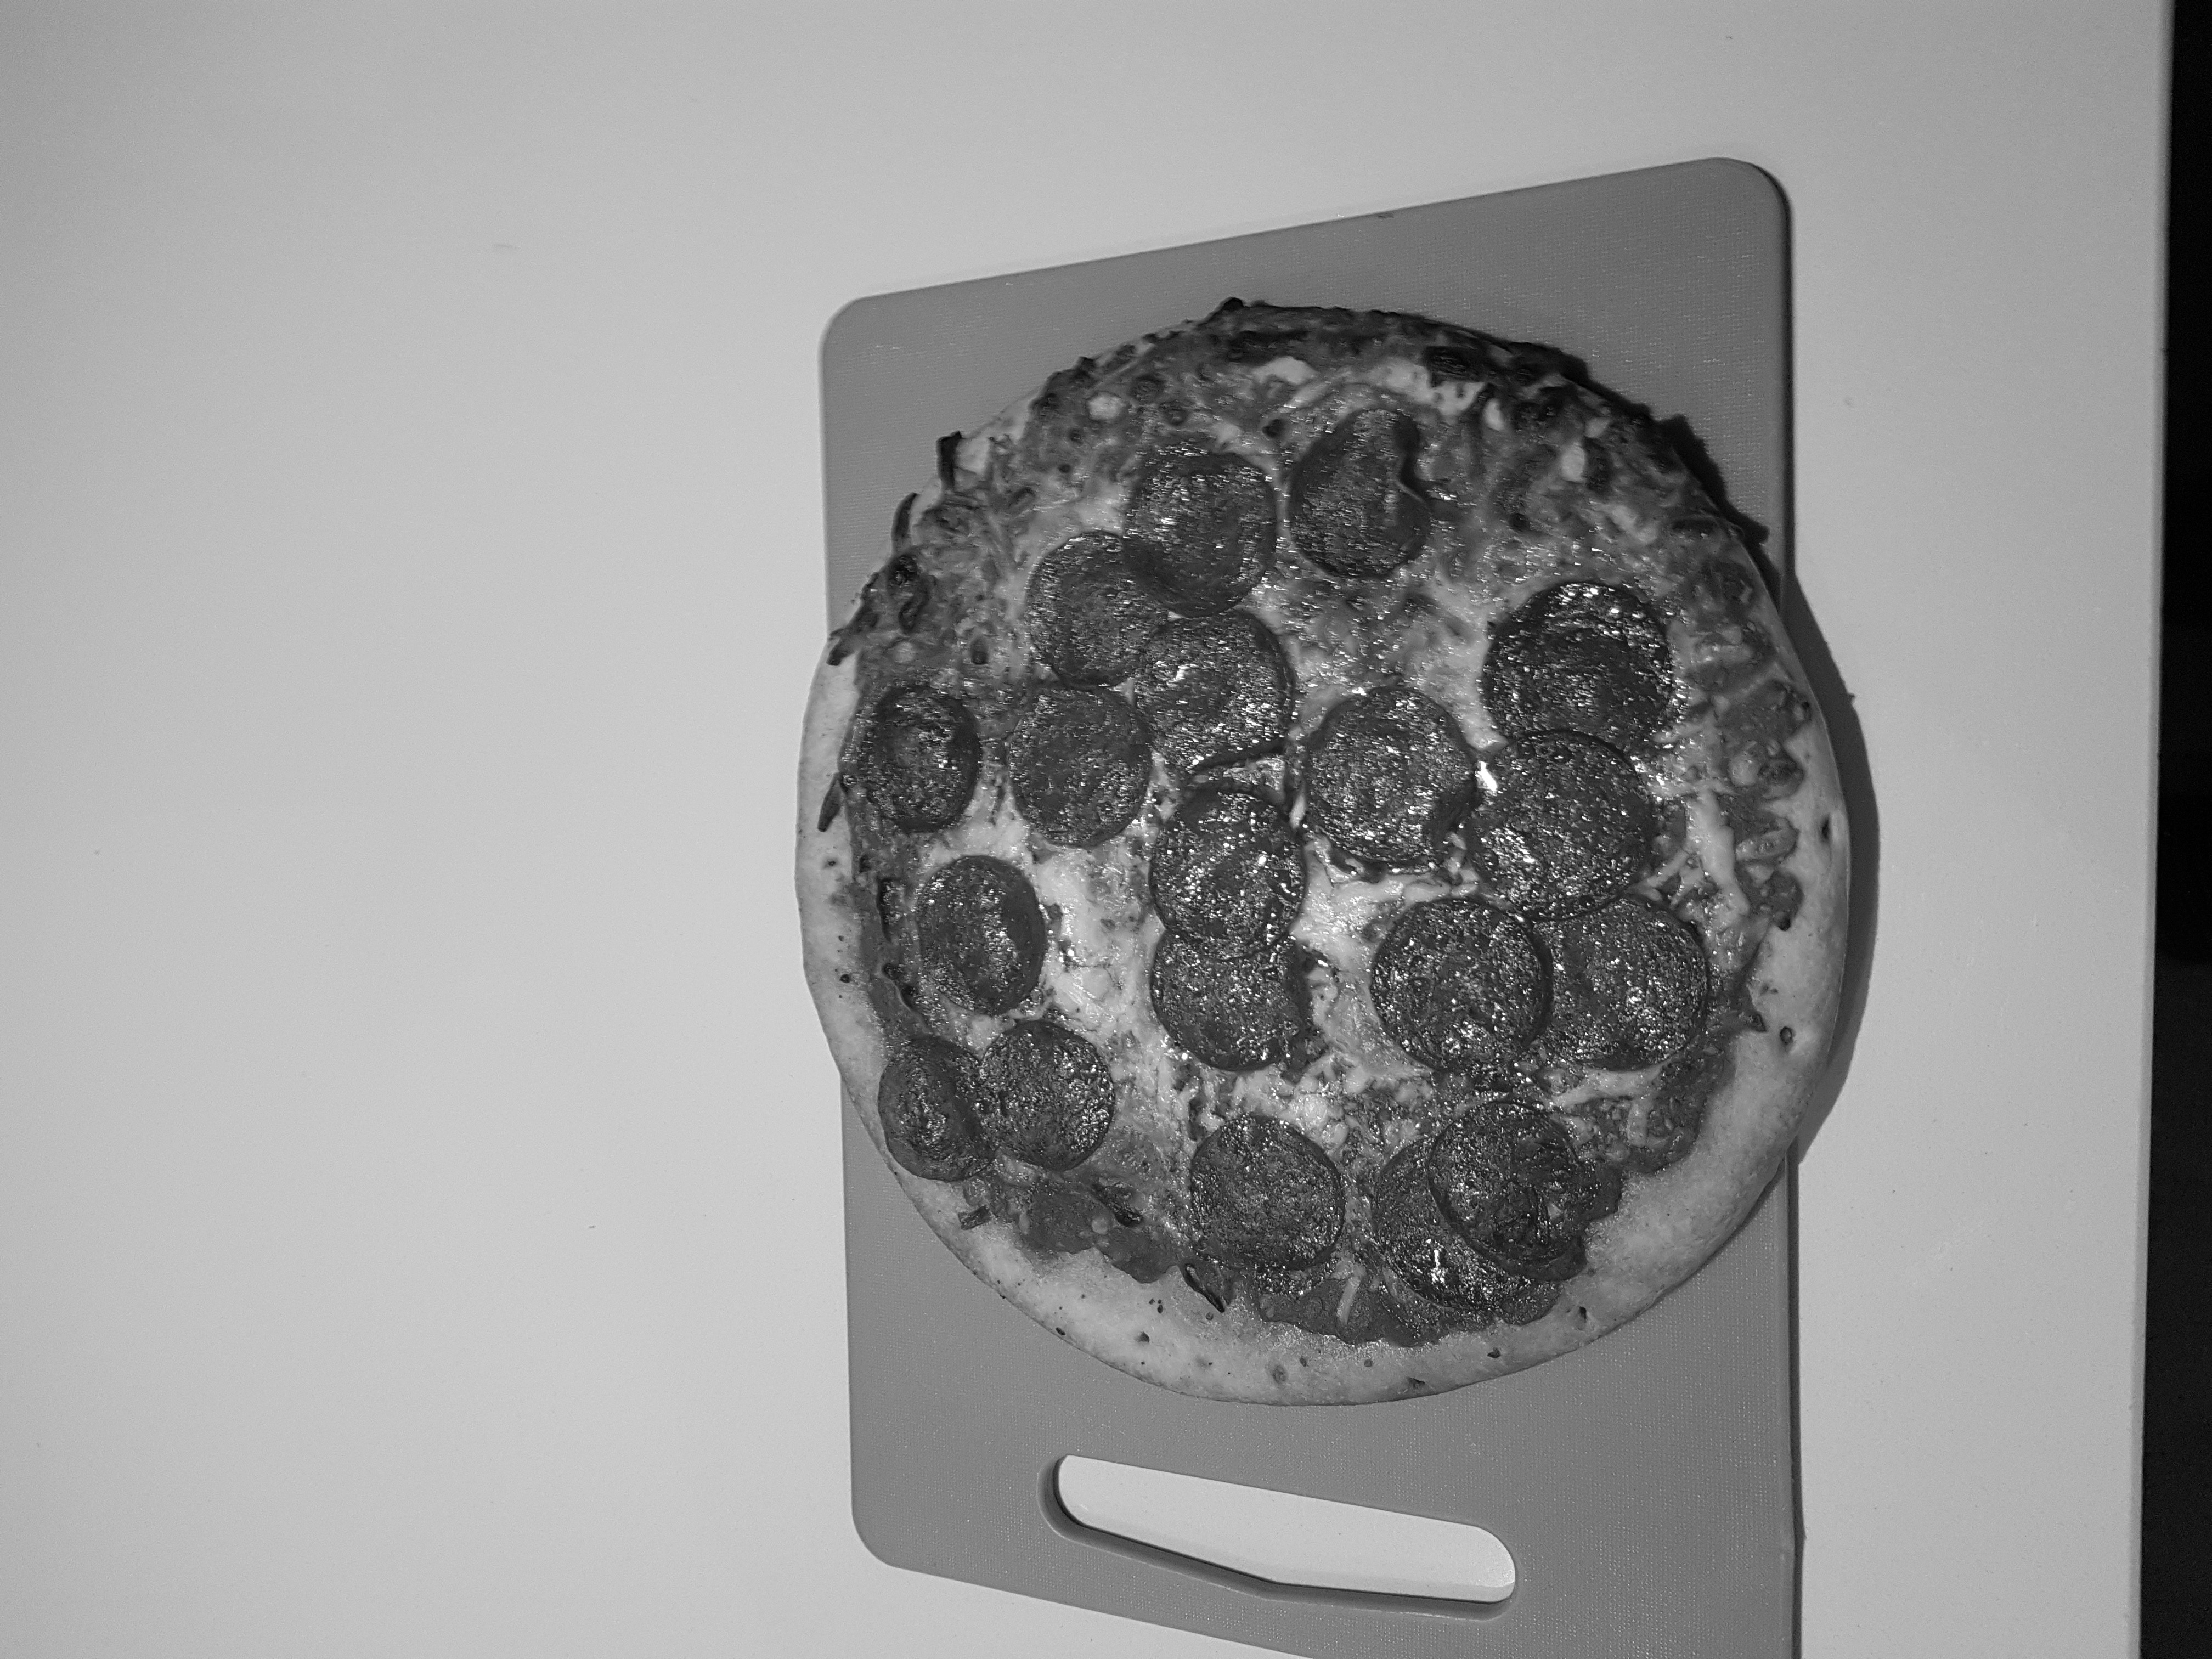
\includegraphics[scale=0.05]{pizza_grey}
    \caption{Pizza Image Greyscale}
    \label{fig:pizzaGrey}
\end{figure}

\tocless\subsection{Results}
The results for this experiment can be seen in Table \ref{colour}.
The 'Top 1' notation in the table suggests that the food was predicted as the number one prediction. The decimal value is the probability of that food type being the correct classification.

\begin{table}[]
\centering
\caption{Effect of Colour}
\label{colour}
\begin{tabular}{|l|l|l|}
\hline
\textbf{Food Image} & \textbf{Pre-Scaled Image} & \textbf{Greyscale}      \\ \hline
Banana     & Top 1 : 0.9971   & Top 1 : 0.9986 \\ \hline
Apple Pie  & Top 1 : 0.7986   & Top 1 : 0.3462   \\ \hline
Pizza      & Top 1 : 0.9753   & Top 2 : 0.1299 \\ \hline
\end{tabular}
\end{table}

\tocless\subsection{Analysis}
\tocless\subsubsection{Colour}
In regard to the images of the banana (Figure \ref{fig:bananaPreRes} and Figure \ref{fig:bananaGrey}), there is very little difference in classification. They were both classified to a Top 1 accuracy and their probabilities differing by only 0.0015 with the grey scale image being of a higher probability. This would indicate that colour is not an important factor for classifying bananas and the coloured image may even have noise. This can be seen in Table \ref{colour}.

The apple pie images (Figure \ref{fig:apple_piePreRes} and Figure \ref{fig:applePieGrey}) were also both classified correctly but with a large gap in the likelihood of that classification being correct. As per Table \ref{colour}, the coloured image had a probability of 0.7986 as opposed to one of 0.3462. This would indicate that while colour is important, there is enough unique data from the rest of the image to result in correct classification.

Finally, the pizza images (Figure \ref{fig:pizzaPreRes} and Figure \ref{fig:pizzaGrey}) were the most contrasting in their results. While the original image was classified to Top 1 accuracy with a likelihood of 0.9753, the coloured image was classified to Top 2 accuracy with a probability of 0.1299. From this we can deduce that colour is vital for the classification of pizza.

Since this experiment only compared three images, we cannot say for sure if this analysis is biased or not.

\tocless\subsubsection{Colour vs Scale}
In the last experiment, it was seen that the pizza and banana images (Figure \ref{fig:pizzaPreRes} and Figure \ref{fig:bananaPreRes}) were not really affected by image quality. While this seems to be true, the image of apple pie, Figure \ref{fig:apple_piePreRes}, was greatly influenced by only being classified to a Top 5 accuracy when down scaled.

For the greyscale images, bananas were not effected greatly and neither was an apple pie but a pizza was greatly influenced.

From this, it can be said that the prominent unique features for each of these food types are different. The banana (Figure \ref{fig:bananaPreRes}) may have focus on shape and texture, the pie (Figure \ref{fig:apple_piePreRes}) on image quality and some influence of colour while the pizza (Figure \ref{fig:pizzaPreRes}) may have a focus on shape, texture and colour.



\section{Visualising Images Through the Network}
\label{visualise}
\tocless\subsection{Overview}
\tocless\subsection{Network Architecture}
\tocless\subsection{Dataset}
\tocless\subsection{API's}
\tocless\subsection{Script}
\tocless\subsection{Results}
\tocless\subsection{Empirical Analysis}


